\documentclass[12pt]{article}
\setlength{\textwidth}{17cm}
\setlength{\textheight}{24cm}
\setlength{\topmargin}{-2cm}
\setlength{\footskip}{1cm}
\setlength{\evensidemargin}{0cm}
\setlength{\oddsidemargin}{0cm}
\setlength{\parindent}{0cm}
\usepackage{amssymb}

\usepackage{allrunes}
\usepackage{amsmath}
\usepackage[magyar]{babel}
\usepackage[T1]{fontenc}
\usepackage[utf8]{inputenc}
\usepackage{fixltx2e}
\usepackage{multirow}

\usepackage[hyphens]{url}
\usepackage[unicode,colorlinks=true,breaklinks]{hyperref}
%\usepackage[dvips]{hyperref}
%should display links, but it does not work with \H accent
%and formulas in section titles

\hypersetup{colorlinks,linkcolor=blue,urlcolor=magenta,citecolor=magenta}
%Breaks long url`s in text, while keeping it one link:

\usepackage{amsfonts}
\usepackage{amsthm}
\usepackage{amssymb}


\theoremstyle{plain}
\usepackage{graphicx}

%\usepackage{gensymb}
\usepackage{float}

% For bra-ket notation
\usepackage{braket}

%% New commands
\newcommand{\dd}{\textrm{d}}

%% Pauli matrices
\newcommand{\sigx}{\sigma_x}
\newcommand{\sigy}{\sigma_y}
\newcommand{\sigz}{\sigma_z}
\newcommand{\xvec}{\mathbf{x}}
\newcommand{\paulix}{
    \left( \begin{array}{cc}
        0 & 1 \\
        1 & 0
    \end{array}
    \right)
}

\newcommand{\pauliy}{
    \left( \begin{array}{cc}
        0 & -i \\
        i & 0
    \end{array}
    \right)
}

\newcommand{\pauliz}{
    \left( \begin{array}{cc}
        1 & 0 \\
        0 & -1
    \end{array}
    \right)
}

\newcommand{\rtor}{
\mathbb{R} \to \mathbb{R}
}

\newcommand{\rmtorm}{
\mathbb{R}^m \to \mathbb{R}^m
}

\begin{document}
\title{6. tétel}
\author{Kaszás Bálint}

\maketitle


\newpage
\begin{abstract}
    Differenciálegyenletek numerikus vizsgálata, Euler-módszer, Runge-Kutta módszer, stabilitás, parciális differenciálegyenletek. Dinamikai rendszerek, kaotikus viselkedés (Complex and Adaptive Dynamical Systems alapján).
\end{abstract}

\section{Differenciálegyenletek numerikus vizsgálata}
A természettudományos, műszaki alkalmazások szempontjából lényeges, folytonos modelleket általában differenciálegyenletek formájában fogalmazzuk meg. Ez azt jelenti, hogy a probléma megoldása során egy olyan függvényt keresünk, amelynek deriváltjai között adott összefüggés érvényes. Aszerint, hogy a keresett függvény milyen változóktól függ, és az előírt összefüggésben milyen deriváltak szerepelnek, elkülönítünk {\em közönséges} és {\em parciális} differenciálegyenleteket. 

Először a közönséges differenciálegyenletek (vagy ODE, ordinary differential equation) felhasználására és numerikus megoldására koncentrálunk. A parciális differenciálegyenletek (PDE, partial differential equation) tárgyalása lényegesen bonyolultabb, ezért ott csak a fő eredményeket közöljük.

Tekintsük tehát a következő közönséges differenciálegyenletet \cite{ode},
\begin{equation}
    \label{1}
    F\left(t, x, \frac{\text{d}x}{\text{d}t}, \frac{\text{d}^2x}{\text{d}t^2}, ..., \frac{\text{d}^{n-1}x}{\text{d}t^{n-1}}\right) = \frac{\text{d}^nx}{\text{d}t^n},
\end{equation}
amely úgy értendő, hogy keressük azt az $x(t) : \rtor$ függvényt, amelynek $t$ változó szerinti deriváltjai között $F$ függvény teremt kapcsolatot. Ekkor (\ref{1}) egy $n$. rendű ODE-t definiál. A keresett $x$ függvény változóját $t$-vel jelöltük, utalva ezzel arra, hogy az alkalmazások szemponjából érdemes erre egy {\em időben változó mennyiségként} gondolni.  Azt az $x(t)$ függvényt, amely a fenti összefüggést kielégíti, a differenciálegyenlet megoldásának hívjuk. A legáltalánosabb ilyen függvény tartalmaz $n$ darab integrálási állandót, ez az egyenlet {\em általános megoldása}. Ebből, az állandók megfelelő megválasztásával, amelyekkel a megoldás illeszkedik előre megadott {\em kezdeti vagy peremfeltételekhez}, kapjuk az egyenlet partikuláris megoldásait. Egyelőre az adott kezdeti feltételekhez illeszkedő megoldás megkeresésére koncentrálunk (kezdeti érték feladat), a peremérték-feladatokat később tárgyaljuk röviden, a parciális differenciálegyenleteknél. 

A fenti egyenlet egyszerűen leképezhető elsőrendű egyenletek rendszerére, az $x_i = \frac{\text{d}^ix}{\text{d}t^i}$ új változó bevezetésével, az $i$. derivált helyett. Ezért a továbbiakban kizárólag elsőrendű differenciálegyenletek rendszerével foglalkozunk, azaz hogyha a különböző változók vektora $\xvec(t)$ : $\mathbb{R} \to \mathbb{R}^n$, akkor
\begin{equation}
    \label{2}
    \frac{\text{d} \xvec(t)}{\text{d}t} = \mathbf{f}(t, \xvec(t)), 
\end{equation}
kiegészítve azzal a kezdeti feltétellel, hogy $\xvec(0) = \xvec_0$ adott vektor. Ezen kezdeti érték feladat megoldására nincs általános módszer, csak nagyon speciális alakú $\mathbf{f}(t, \xvec)$ függvények mellett ismert a megoldás explicit alakja (például ha $\mathbf{f}$ lineáris $\xvec$-ben). A legtöbbször azonban muszáj numerikus módszerekre hagyatkozni. Ezek azt a tulajdonságot használják ki, hogy az ODE-k széles osztálya \footnote{A Picard–Lindelöf tétel\cite{ode} globális megoldhatóságot garantál: Amennyiben $\mathbf{f}$ Lipschitz folytonos $\xvec$ szerint, és folytonos $t$ szerint, akkor van olyan időintervallum, amelyen tetszőleges $\xvec_0$ kezdeti értékhez tartozó megoldás létezik és egyedi. (Lipschitz-folytonosság: Bármely $t$-re, és $\forall$ $\xvec_1, \xvec_2$ $\in$ $\mathbb{R}^n$, $\exists K>0$ $||\mathbf{f}(t,\xvec_1) -\mathbf{f}(t, \xvec_2)||\leq K||\xvec_1 - \xvec_2||$)}, adott kezdeti feltétel mellett egyértelmű megoldással rendelkezik. Ez azt teszi lehetővé, hogy az adott kezdeti feltételből indulva, kis időlépéseket téve göngyölítsük fel a megoldást. 
\subsection{Explicit és implicit módszerek}
A numerikus megoldás előállításához diszkrét időközönként, $t_n = t_0 + nh$ időpontokban keressük a megoldás $\xvec(t_n)$ pontjait, ahol $t_0$ a kezdő időpont és $h$ a lépésköz. 
A feladat az, hogy $\xvec(t_{n+1})$ pontot kifejezzük a korábbi pillanatbeli $\xvec(t_n)$ értékkel, feltéve hogy (\ref{2}) jobb oldalát, $\mathbf{f}$-et is ismerjük. Ez a megközelítés az úgynevezett {\em explicit módszer}, mert egy explicit kifejezést használunk, amely $\xvec(t_{n+1})$-et megadja. Ennél általánosabbak (és robosztusabbak) az {\em implicit módszerek}, amelyek csak egy $G(\xvec(t_n), \xvec(t_{n+1}))=0$ alakú implicit összefüggést követelnek meg. A tapasztalat szerint azonban a problémák többségében elegendő explicit módszereket használni \cite{landau, tel}.

Minden, a továbbiakban tárgyalt explicit módszert úgy kapunk, hogy $\xvec(t_{n+1})=\xvec(t_n + h)$-t Taylor-sorba fejtjük, azaz
\begin{equation}
\label{3}
    \xvec(t_{n+1}) = \xvec(t_n) + \sum_{i=1}^{\infty} \frac{1}{i!}\frac{\text{d}^i \xvec(t_n)}{\text{d}t^i}h^i.
\end{equation}
Ezt követően a megoldás deriváltjait a differenciálegyenlet, (\ref{2}) alapján fejezzük ki. 
\subsection{Euler módszer}
A legegyszerűbb közelítést akkor kapjuk, hogyha a (\ref{3}) Taylor-sorfejtést mindössze első rendig tekintjük. Ekkor, felhasználva a differenciálegyenletet,
\begin{equation}
    \label{euler}
    \xvec(t_{n+1}) = \xvec(t_n) + h\mathbf{f}(t_n, \xvec(t_n)),
\end{equation}
adódik. Ismert az is, hogy az elkövetett hiba $h^2$-el arányos. Az Euler-módszer hátránya, hogy ha elég pontos közelítést szeretnénk kapni, nagyon kis $h$ lépésközt kell választanunk. Ezzel azonban a megtett lépések számát növeljük, aminek következtében az egy lépésben elkövetett numerikus, kerekítési hibák gyorsan felnövekedhetnek \cite{landau}. 
\subsection{Runge-Kutta módszer}
A Runge-Kutta módszerekre a Taylor-sorfejtés magasabb rendű tagjai vezetnek. Másodrendnél megállva, $\frac{\text{d}^2\xvec}{\text{d}t^2}$-et a differenciálegyenlettel kifejezve kapjuk a következő, {\em másodrendű Runge-Kutta módszert}. 
\begin{align}
    \xvec(t_{n+1}) &= \xvec(t_n) +  \frac{1}{2}(\mathbf{k_1} + \mathbf{k_2}), \\
    \mathbf{k_1} = h \mathbf{f}(t_n, \xvec(t_n))&,   \qquad   \mathbf{k_2} = h \mathbf{f}(t_n+h, \xvec(t_n) + \mathbf{k_1}).
\end{align}
Itt az egy lépésben elkövetett hiba már csak $h^3$ rendű. A folyamat elméletileg tetszőleges rendig folytatható, de a gyakorlatban a {\em negyedrendű} Runge-Kutta módszer már jó kompromisszumnak. Ezt a következő összefüggések definiálják 
\begin{align}
    \xvec(t_{n+1}) &= \xvec(t_n) +  \frac{1}{6}(\mathbf{k_1} + 2\mathbf{k_2} + 2\mathbf{k_3} + \mathbf{k_4}), \\
    \mathbf{k_1} = h \mathbf{f}(t_n, \xvec(t_n))&,   \qquad   \mathbf{k_2} = h \mathbf{f}\left(t_n+h/2, \frac{\xvec(t_n)+ \mathbf{k_1}}{2}\right) \\
    \mathbf{k_3} = h \mathbf{f}(t_n/2, \xvec(t_n)+ \mathbf{k_2}/2)&,   \qquad   \mathbf{k_4} = h \mathbf{f}(t_n+h, \xvec(t_n)+ \mathbf{k_3}).
\end{align}
Ezzel a negyedrendű módszerrel a lépésenkénti hiba $h^5$ nagyságrendű. Ugyan a számítási igény is nagyobb (lépésenként 4-szer kell kiértékelni $\mathbf{f}$-et), elegendő kisebb $h$ lépésközt választani a kellő precizitás eléréséhez. 

További általánosítást jelentenek az adaptív lépésközös Runge-Kutta algoritmusok. Legismertebb az ú. n. Runge-Kutta-Fehlberg módszer. Ehhez, egyetlen lépést a negyed- és az ötödrendű Runge-Kutta módszerrel egyszerre számolva teszünk meg. A magasabb rendű módszer segítségével megbecsülhető a lépés során elkövetett hiba. Amennyiben ez a numerikus integrálás során egy előre definiált korlátot túllép, a {\em lépésköz csökkentését} követően megismételjük a hibás lépést. 
\subsection{A módszerek stabilitása}
Fontos kérdés, hogy a választott numerikus módszer milyen feltételek mellett, vagy milyen lépésközök esetén marad numerikusan stabil. Azokat a rendszereket, amelyek tipikusan instabillá válnak, általában {\em stiff}-nek hívjuk. Pontos definíció közlése nélkül azon problémák stiffek, amelyek megoldásai gyorsan változnak egy tartományon. 

A numerikus ODE megoldó algoritmusok stabilitását a következő prototipikus egyenleten keresztül szokás vizsgálni
\begin{equation}
\label{test}
    \frac{\text{d}y}{\text{d}x} = k y.
\end{equation}
Az egyenlet megoldásai nullához tartanak, amennyiben $k<0$. A numerikus módszer stabil, hogyha a közelítő $y_n$-ek sorozata is nullához tart. Alkalmazzuk (\ref{test})-re az Euler-módszert. Indukcióval belátható, hogy a megoldás numerikus közelítése 
$$
y_n = y_0(1+hk)^n,
$$
ahol $y_0 = y(0)$, a kezdőfeltétel. Látható, hogy az $y_n$ sorozat akkor tart nullához, ha teljesül $|1 + hk| < 1$, ami a stabilitás feltételét adja. Azt is mondhatjuk tehát, hogy ez az egyenlet stiff, mert a stabilitáshoz rendkívül kicsi lépésközzel kellene közelítenünk a megoldást. 

Az ilyen, stiff egyenletek kezelésére alkalmasak a fent már említett {\em implicit módszerek}. Itt csak a legegyszerűbb esetet tárgyaljuk, az implicit Euler módszert, amit a következő összefüggés definiál

\begin{equation}
\label{beuler}
    \xvec(t_{n+1}) = \xvec(t_n) + h\mathbf{f}(t_{n+1}, \xvec(t_{n+1})).
\end{equation}
Mivel azonban a keresett $\xvec(t_{n+1})$ az egyenlet mindkét oldalán szerepel, itt minden lépésben egy algebrai egyenletet kell megoldani (például Newton-Raphson módszerrel \cite{landau}). Belátható, hogy az implicit Euler-módszert alkalmazva (\ref{test}) egyenletre, a stabilitási feltétel $1/|1 + hk| < 0$, ami viszont tetszőleges $h>0$-ra teljesül (feltéve hogy $k<0$).  
\subsection{Parciális differenciálegyenletek}
A parciális differenciálegyenletek (a közönségesekkel ellentétben) a keresett függvény egynél több változója szerinti parciális deriváltjait is tartalmazhatják. Legtöbbször a keresett függvény egy fizikai skalármező $U(x, y, z, t)$ amely egyszerre függ a helytől és az időtől is. A dinamikát leíró egyenleten túl a problémát a peremfeltétel megadása egészíti ki. A PDE-k esetén nincsen olyan egyszerűen megfogalmazható feltétel, amely garantálná a megoldás létezését és jól definiáltságát, sokszor fizikai intuícióra kell hagyatkozni (például, hogy elég peremfeltételt adtunk-e meg). 

Éppen ezért a numerikus megoldásra, nincsen olyan egyszerű, explicit módszer mint ami az ODE-knél rendelkezésre állt. A legegyszerűbb megoldási módszer az, hogy az egyenletben szereplő deriváltakat véges különbségekkel helyettesítjük, ez az úgynevezett {\em véges differenciák módszere, vagy FDM}. Az általános leírás helyett célszerű egy egyszerű példán bemutatni a megoldás menetét. Tekintsük tehát a 2 dimenziós Laplace egyenletet, 
\begin{equation}
    \label{2dlap}
    \frac{\partial ^2 U}{\partial x^2}  + \frac{\partial ^2 U}{\partial y^2} = 0.
\end{equation}
Ahol a keresett függvény $U(x,y)$. Sorba fejtve, $U(x+\Delta x, y)$ és $U(x - \Delta x, y)$ közelítéséből adódik,

\begin{align}
  U(x + \Delta x, y) &= U(x, y) + \frac{\partial U}{\partial x}\Delta x + \frac{1}{2}\frac{\partial ^2 U}{\partial x^2}\Delta x^2 + ... \\
    U(x + \Delta x, y) &= U(x, y) - \frac{\partial U}{\partial x}\Delta x + \frac{1}{2}\frac{\partial ^2 U}{\partial x^2}\Delta x^2 - ...
    \end{align},
mely két egyenletet kivonva egymásból véges közelítését kapjuk a második deriváltnak.

\begin{equation}
\label{fdm}
\frac{\partial ^2 U}{\partial x^2} = \frac{U(x + \Delta x, y) + U(x- \Delta x, y) - 2U(x,y)}{\Delta x ^2}.
\end{equation}
Elismételve az $y$ irányban is, és feltételezve hogy $\Delta x = \Delta y = \Delta$, kapjuk a Laplace egyenlet véges differencia-közelítését.
\begin{equation}
    \label{lapfdm}
    U(x + \Delta, y) + U(x - \Delta, y) + U(x, y+ \Delta) + U(x, y - \Delta) - 4 U(x, y) = 0. 
\end{equation}
Ennek ismeretében, az egyenletet $U(x,y)$-ra rendezve, minden pontban kiszámolhatjuk $U$ értékét, a körülötte $\Delta$ távol lévő pontokban mért értékek segítségével. Ezt a gyakorlatban iteratívan végezzük, azaz egy  kezdeti $U(x,y)$ függvényből indulva, lépésenként minden pontban {\em frissítjük} $U(x,y)$ aktuális értékét, a (\ref{lapfdm}) egyenlet szerint. 

Az itt vázolt iterációs módszert valamennyivel gyorsítja, ha a Successive Overrelaxationt (SOR) \cite{landau} alkalmazzuk. Az adott iterációs lépésben, az $(x,y)$ pontban legyen $r(x,y) = U^{n+1}(x,y) - U^{n}(x,y)$ az a szám, amivel frissíteni kell $U(x,y)$ értékét ($n$ index számozza az iterációk számát). A SOR algoritmus szerint ilyenkor az $U^{n+1}(x,y) = U^{n}(x,y) + \omega r(x,y)$ iterációt alkalmazhatjuk, amely gyakran stabil $1<\omega < 2$-re, és nagyban gyorsítja a konvergenciát. 
\section{Dinamikai rendszerek}
A dinamikai rendszerek elmélete, a fent tárgyalt differenciálegyenletek alkalmazása valós, időben változó problémákra \cite{tel, compl}. Egy dinamikai rendszert a 
\begin{equation}
    \label{dyn}
    \frac{\text{d} \xvec(t)}{\text{d}t} = \mathbf{f}(t, \xvec(t)) 
\end{equation}
egyenlet definiál. A rendszer változói $(x_1, x_2, x_2, ..., x_n) = \xvec$ által kifeszített teret hívjuk a rendszer {\em fázisterének}. Az ebben leírt $\xvec(t)$ görbe, amely megoldása (\ref{dyn})-nek, pedig a rendszer egyik {\em trajektóriája}. A továbbiakban ezen trajektóriák közül, valamilyen kitűntetett viselkedést mutatókra fogunk koncentrálni. Az egyszerűség kedvéért {\em autonóm} rendszereket fogunk tekinteni, amelyben a dinamika nem függ explicite az időtől, így $\mathbf{f}$ $t$ függését el is hagyjuk. 

A legfontosabb speciális trajektóriák a {\em fixpontok}. Ezek a dinamika invariáns pontjai a fázistérben, azaz $\mathbf{f(\xvec(t))} = 0$. Egy fixpontot {\em stabilnak} mondunk, ha a környező trajektóriákat vonzza, és {\em instabilnak}, ha a azokat taszítja. 
Példának tekintsük az alábbi, két dimenziós dinamikai rendszert, polárkoordinátákban felírva, azaz $x(t) = r(t)\cos(\varphi(t))$ és $y(t) = r(t)\sin(\varphi(t))$.
\begin{align}
    \label{rot}
    \frac{\text{d} \varphi}{\text{d}t} &= \omega \\
    \frac{\text{d} r}{\text{d}t} &= (\gamma - r^2)r
\end{align}
A rendszerben szerepel egy $\gamma$ paraméter is, amely drasztikusan  befolyásolja a dinamikát: $\gamma < 0$ esetén a hosszú távú viselkedést az $x=y=0$ fixpont határozza meg, míg $\gamma = r_c^2 > 0$-ra egy oszcilláló megoldás jelenik meg, amelynek sugara pont $r_c$. Ezt a periodikus trajektóriát {\em határciklusnak} hívják. 

\begin{figure}[h!]
    \centering
    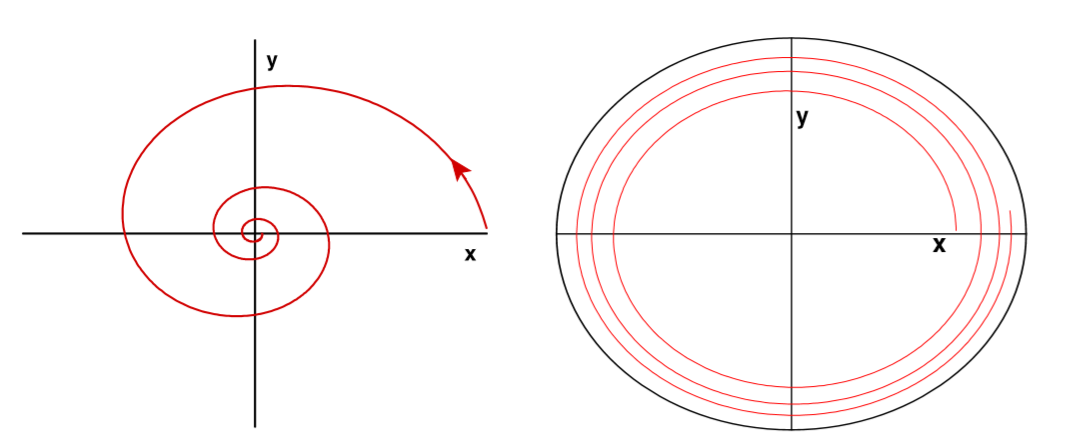
\includegraphics[width = 0.6\textwidth]{media/rotation.png}
    \caption{A fenti ($\varphi$, $r$) rendszer két tipikus, hosszú távú viselkedését mutató trajektóriák, az $x, y$ síkon szemléltetve. A bal oldalon $\gamma<0$ esetén, az $x=y=0$ fixponthoz való konvergenciát látjuk. A jobb oldalon pedig $\gamma=r_c^2>0$ esetén kialakuló $r_c$ sugarú periodikus határciklust. }
    \label{fig:rot}
\end{figure}
A példaként felírt rendszerben $\gamma=0$ paraméter értéknél egy drasztikus átmenetet látunk. Azt mondjuk, hogy $\gamma = 0$-nál {\em bifurkáció} történik\footnote{A határciklus viselkedés megjelenése ú. n. Hopf-bifurkációval történik \cite{compl}}.

Fontos még megemlíteni, hogy bizonyos esetekben, a dinamikai rendszerekhez lehet társítani olyan mennyiségeket, amelyek állandóak egy adott trajektória mentén. A klasszikus mechanikai motiváció miatt ezeket gyakran {\em mozgásállandónak} hívják. Általánosan elmondható, hogy amennyiben egy rendszer sok mozgásállandóval rendelkezik, a megoldást egy {\em explicit integrál} kiszámításával kapjuk. Ezért, az elegendő mozgásállandóval rendelkező rendszereket {\em integrálhatónak} hívjuk. A nem integrálható rendszerekre ezzel ellentétben sokkal bonyolultabb, kaotikus viselkedés is jellemző. 
\subsection{Kaotikus viselkedés}
A huszadik század végére tisztává vált, hogy az integrálható rendszerek sokkal inkább kivételek, egy általános dinamikai rendszer sokkal bonyolultabb viselkedést mutat. A kaotikus rendszerek annyira érzékenyek a numerikus pontatlanságokra, hogy viselkedésük egyáltalán nem jelezhető előre, annak ellenére hogy az őket leíró differenciálegyenletek teljesen {\em determinisztikusak}.

Pontosabban megfogalmazva, a kaotikus rendszereket a kezdőfeltételre jellemző {\em exponenciális} érzékenység definiálja. Azaz, a kezdőfeltételben lévő kezdeti hiba időben exponenciálisan növekszik. 

Az egyik legegyszerűbb példája a kaotikus rendszereknek a {\em logisztikus leképezés}. Az eddigiekkel ellentétben most nem folytonos idejű, differenciálegyenlettel adott rendszerről lesz szó, hanem egy diszkrét idejű leképezésről, amelyet a következő formula definiál
\begin{equation}
    x_{n+1} = rx_n(1-x_n), \qquad \qquad x_n \in [0,1], r\in [0,4].
\end{equation}
Értelmezhetjük úgy, hogy az $x_n$ változó egy faj egyedeinek számát jelenti az $n.$ évben. Minden egyednek $r(1-x_n)$ számú utóda van évente. A rendszer $r$ bizonyos értékeire rendkívül bonyolult, kaotikus viselkedést képes mutatni. 

Ezt láthatjuk, ha megvizsgáljuk a rendszer fixpontjait, vagyis azokat az $x_n$ értékeket, amelyeknél a dinamika stabilizálódik hosszú idő után. Azon tulajdonságú $x$ pontokat keressük, amelyre ($n$-től függetlenül) $x = rx(1-x)$.

A nemtriviális megoldás $r(1-x) = 1$-ből adódik, amely $x^{(1)} = 1- 1/r$, amennyiben $r>r_1=1$, vagyis egy bifurkációt látunk $r_1=1$ értéknél, amelynél megjelenik a fixpont. 

A stabilitását megvizsgálva kiderül, hogy van egy $r_2$ érték, melyre a fixpont $r>r_2$  esetén már elveszíti a stabilitását, a hozzá közeli pontokat {\em taszítani kezdi}.

Ebben az $r_2$ bifurkációs pontban olyan új megoldások születnek (méghozzá kettő), amely a {\em kétszeresen iterált leképezésnek} fixpontja, vagyis {\em kettes ciklus}, $x_{n+2} = x_n$. A kettes ciklusnak is kiszámítható a stabilitási tartománya, amely addig tart, amíg a {\em négyszeresen iterált} leképezés fixpontjai, a {\em négyes ciklusok} megjelennek. 

Általánosan elmondható, hogy $r$ növelésével egyre nagyobb rendű ciklusok jelennek meg, mindig megduplázva az addig stabil ciklus periodicitását. $2^{n-1}$ darab megoldást találunk, amely a $2^{n-1}$-szer iterált leképezésnek fixpontja, vagyis $2^{n-1}$-es ciklus. Ezeknek pedig kiszámítható a stabilitási tartománya, amely valamely $r_n < r < r_{n+1}$ intervallum. A logisztikus leképezés esetén az $r_n$ sorozatnak van határértéke, 
\begin{equation}
    \lim_{n \to \infty} r_n = r_{\infty} = 3.5599456...,
\end{equation}
ezen $r$ érték fölött {\em végtelen} periódusú instabil ciklusok jönnek létre, ami azt jelenti hogy a rendszer {\em soha} nem tér vissza a kezdeti értékére. A végtelen számú instabil pálya által uralt dinamika kaotikussá válik, és megjelenik a kezdőfeltételekre való exponenciális érzékenység.

Ezt számszerűsíti a {\em Lyapunov-exponens}. Vegyünk két trajektóriáját a logisztikus leképezésnek, amelyek $x_0$ és $y_0$ pontokból indulnak. A dinamika során ezek eltávolodhatnak egymástól vagy közeledhetnek egymáshoz, a közöttük lévő $|x_n - y_n|$ távolság $\sim \text{exp}(\lambda n)$ szerint változik, ahol $\lambda$ a Lyapunov-exponens. Ezzel megfogalmazhatjuk, hogy a $\lambda > 0$-val jellemezhető viselkedést hívjuk kaotikusnak. A \ref{fig:lyap}. ábra a logisztikus leképezés ciklusait, és az ezekhez tartozó Lyapunov-exponenseket mutatja, az $r$ paraméter függvényében.

\begin{figure}[h!]
    \centering
    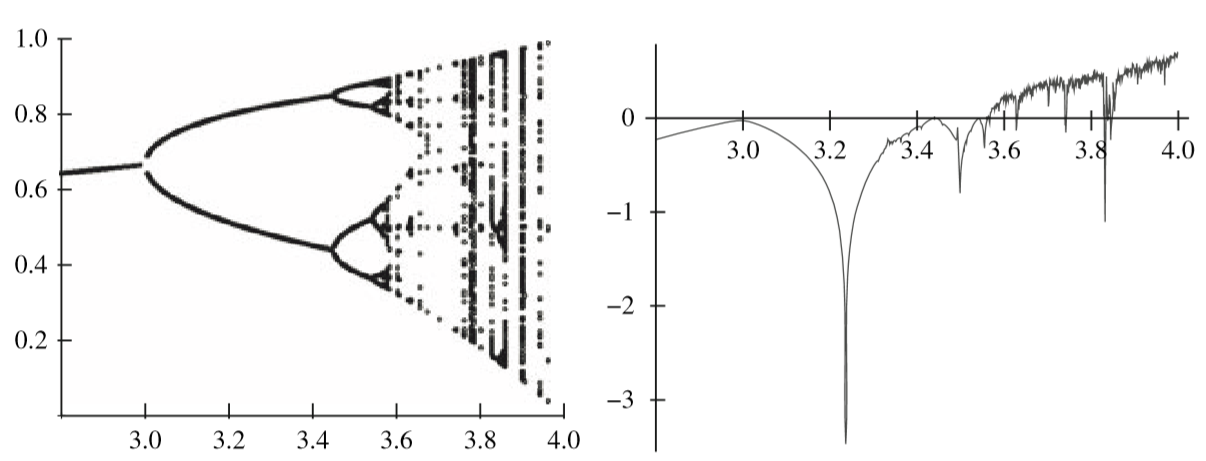
\includegraphics[width = 0.7\textwidth]{media/lyap.PNG}
    \caption{A bal panelen a logisztikus leképezés bifurkációs diagramja látható, vagyis a rendszer stabil pályáinak koordinátái, $r$ függvényében. A jobb panelen pedig ugyanazen $r$ értékek mellett számolt Lyapunov-exponensek láthatók. A pozitív $\lambda$-jú tartományokban kaotikus viselkedést tapasztalunk. }
    \label{fig:lyap}
\end{figure}
\newpage
\bibliographystyle{plain}
\bibliography{references}

\end{document}